\documentclass{beamer}

\newcommand{\st}{\texttt{serpentTools} }
\title{The \texttt{serpentTools} python package}
\author{Andrew Johnson}
\date{4 April, 2016}

\usepackage{multicol}
\usepackage{graphicx}
\usepackage{hyperref}
\hypersetup{
    colorlinks=true,
    linkcolor=black,
    urlcolor=orange
}
\usepackage{tikz}
\usepackage{color}
\usepackage{listings}

\begin{document}

\begin{frame}
\titlepage
\end{frame}

\section*{Outline}
\begin{frame}{Outline}
    \begin{multicols}{2}
        \tableofcontents[hideallsubsections]
    \end{multicols}
\end{frame}

\begin{frame}{Before we dive in...}
    \begin{itemize}
        \item{Output files and content available at \url{https://github.com/drewejohnson/ans-student19-serpenttools}}
        \item Will be using \href{https://jupyter.org/}{Jupyter notebooks} for examples
        \item Python 2.7, or 3.5+
        \item Can use \texttt{numpy}, \texttt{matplotlib} inside from python
            \begin{itemize}
                \item Either in a Python/iPython environment or Jupyter notebook
            \end{itemize}
        \onslide<2->
        \item{Who has used SERPENT/MCNP before?}
        \onslide<3->
        \item{Python}
    \end{itemize}
\end{frame}

\section{Objectives}

\begin{frame}{Objectives}
    \begin{itemize}
        \item Moderate familiarity with the SERPENT Monte Carlo code
        \begin{itemize}
            \item Basic structure
            \item ``Best'' practices
        \end{itemize}
        \item Detailed familiarity with \st API
        \item Explore some applications built with \st
    \end{itemize}
\end{frame}

\section{SERPENT}
\begin{frame}{SERPENT}
    \begin{itemize}
        \item Monte Carlo code developed and distributed by VTT Technical Research Centre of Finland, LTD
        \item Criticality and fixed-source calculations
        \item Reactor physics oriented, but general applications
        \item Support for detectors (tallies), depletion, homogenization, and more
    \end{itemize}
\end{frame}

\begin{frame}{SERPENT Resources}
    \begin{itemize}
        \item{Main website - \url{http://montecarlo.vtt.fi}}
        \item{Wiki / Online manual - \url{http://serpent.vtt.fi/mediawiki/index.php/Main_Page}}
        \item{Discussion board - \url{https://ttuki.vtt.fi/serpent/}}
    \end{itemize}
\end{frame}

\begin{frame}{Sample output}
    \begin{figure}
        \centering
        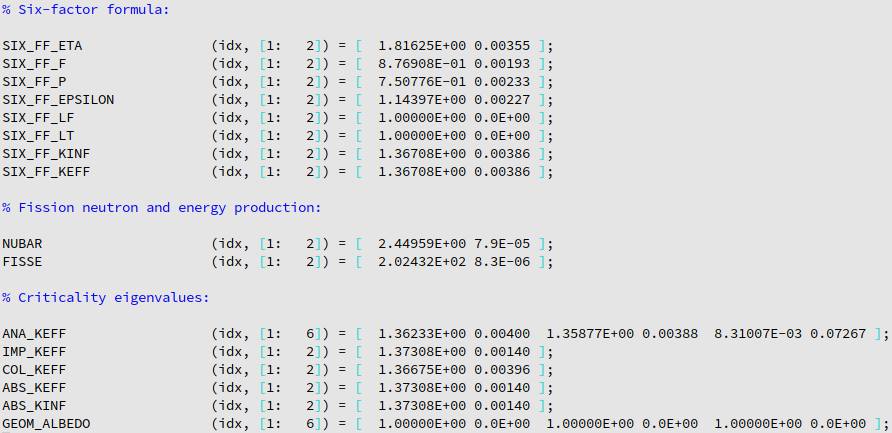
\includegraphics[width=\linewidth]{./images/res.png}
        \caption{Selection of main results files}
    \end{figure}
\end{frame}

\section{\st}

\begin{frame}{Motivation}
    \begin{itemize}
        \item MATLAB is expensive (for non-students)\footnote{FOSS alternative: Octave}
        \item Complicated and connected data stored as arrays
        \item For large problems, output files can cripple MATLAB
        \begin{itemize}
            \item Full core depletion
            \item Many burnup steps
            \item Thousands of burnable materials
            \item $\rightarrow$ 10,000+ arrays with 1000+ items
            \item $\rightarrow O(100)$ MB \textit{text file}
        \end{itemize}
    \end{itemize}
\end{frame}

\begin{frame}{\st}
    \begin{itemize}
        \item Open-source python package for expediting analysis with SERPENT
        \item Builds off of \texttt{numpy}, \texttt{matplotlib}, and \texttt{scipy}
        \item Designed for speed, control, and flexibility
        \item Publication-quality plots in a few commands
    \end{itemize}
\end{frame}


\begin{frame}{\st Resources}
    \begin{itemize}
        \item GitHub Repo - \url{https://github.com/CORE-GATECH-GROUP/serpent-tools}
        \item Documentation - \url{https://serpent-tools.readthedocs.io/en/master/}
    \end{itemize}
\end{frame}

\begin{frame}{Installation}
    \begin{itemize}
        \item Install Guide - \url{https://serpent-tools.readthedocs.io/en/master/install.html}
        \item Easy install
            \begin{itemize}
                \item Open terminal
                \item \texttt{\$ pip install serpentTools [--user] [--pre]}
            \end{itemize}
        \item Windows - use \href{https://www.anaconda.com/distribution/}{Anaconda}
            \begin{itemize}
                \item Open Anaconda Prompt
                \item \texttt{\$ conda install numpy matplotlib scipy pyyaml}
                \item \texttt{\$ pip install serpentTools}
            \end{itemize}
    \end{itemize}
\end{frame}

\section{Simple Input File}

\begin{frame}{Simple Input File}
    \tableofcontents[sectionstyle=show/hide,subsectionstyle=show/show/hide]
\end{frame}

\begin{frame}{Basic input commands}
    \begin{itemize}
        \item Input is very free-form and flexible
        \item Many settings follow \texttt{set <name> <options>} syntax
        \item Uses CSG for geometry like MCNP
        \begin{itemize}
            \item surfaces, cells, lattices, universes
        \end{itemize}
        \item Materials are assigned isotopes and properties
        \begin{itemize}
            \item volume, density, temperature, etc.
        \end{itemize}
    \end{itemize}
\end{frame}

\subsection{Geometry}

\begin{frame}{Pin macro}
    \begin{itemize}
        \item{Handy shortcut for defining fuel pins}
        \item{Basic syntax: \texttt{pin <name> <m1> <r1> <m2> <r2> ... <mN>}}
        \item{Each material is placed from previous radius to next radius}
        \onslide<2->
        \item{\texttt{pin fp \textcolor{red}{fuel} 0.39 \textcolor{green}{clad}
               0.45 \textcolor{blue}{water}}}
    \end{itemize}
    \begin{figure}
        
\begin{tikzpicture}[scale=3]
            \filldraw[blue] (-0.63cm, -0.63cm) rectangle (0.63cm,0.63cm);
            \filldraw[green] (0,0) circle (0.45cm);
            \filldraw[red] (0, 0) circle (0.39cm);
        \end{tikzpicture}
    \end{figure}
\end{frame}

\begin{frame}{Lattice}
    \begin{itemize}
        \item{Many lattice types}
        \begin{itemize}
            \item{XY Cartesian, vertical, hexagonal, etc.}
        \end{itemize}
        \item{Place pins in Cartesian grid}
        \item{\texttt{lat <univ> 1 x0 y0 nx ny \textcolor{red}{pitch}}}
        \onslide<2->
        \item{\texttt{lat 100 1 0 0 6 6 \textcolor{red}{1.3} fp fp fp fp ...}}
    \end{itemize}
    \begin{figure}
        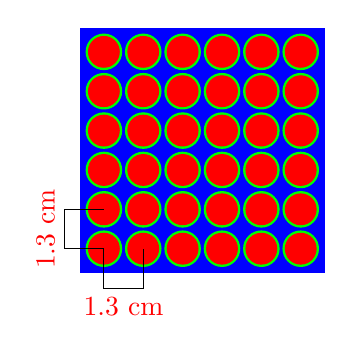
\begin{tikzpicture}[scale=0.5]
            \filldraw[blue] (-3.1, -3.1) rectangle (3.1, 3.1);
            \foreach \x in {-2.5,...,2.5}
                \foreach \y in {-2.5,...,2.5} {
                    \filldraw[green,xshift=\x cm,yshift=\y cm] circle (0.45cm);
                    \filldraw[red,xshift=\x cm,yshift=\y cm] circle (0.39cm);
                }
            \draw (-2.5, -2.5) -- (-2.5, -3.5) -- node[below,red] {1.3 cm} (-1.5, -3.5) -- (-1.5, -2.5);
            \draw (-2.5, -2.5) -- (-3.5, -2.5) -- node[sloped, above,red] {1.3 cm} (-3.5, -1.5) -- (-2.5, -1.5);
        \end{tikzpicture}
    \end{figure}
\end{frame}

\begin{frame}{Simple Surfaces}
    \begin{itemize}
        \item{Many options for building geometric surfaces}
        \item{Used to define boundaries to materials, universes, etc.}
        \item{Simple square: \texttt{surf <id> sqc x0 y0 hp [rad]}}
        \onslide<2->
        \item{\texttt{surf \textcolor{red}{10} sqc 0 0 3.9 0.2}}
        \item{\texttt{surf \textcolor{blue}{11} sqc 0 0 4.5}}
    \end{itemize}
    \begin{figure}
        \centering
    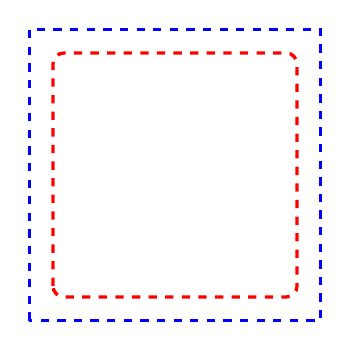
\begin{tikzpicture}[scale=0.5]
        \draw[blue,very thick,dashed] (-3.7, -3.7) rectangle (3.7, 3.7);
        \draw[rounded corners,red,very thick,dashed] (-3.1, -3.1) rectangle (3.1, 3.1);
    \end{tikzpicture}
    \end{figure}
\end{frame}

\begin{frame}{Cells}
    \begin{itemize}
        \item{Cells are defined by intersections, unions of surfaces}
        \item{\texttt{cell <id> <univ> [what] [surf boundaries]}}
        \onslide<2->
        \item{\texttt{cell 1 0 fill 100 -\textcolor{red}{10}}}
        \item{\texttt{cell 2 0 \textcolor{green}{clad} \textcolor{red}{10} -\textcolor{blue}{11}}}
        \item{\texttt{cell 3 0 outside \textcolor{blue}{11}}}
    \end{itemize}
    \begin{figure}
        \centering
        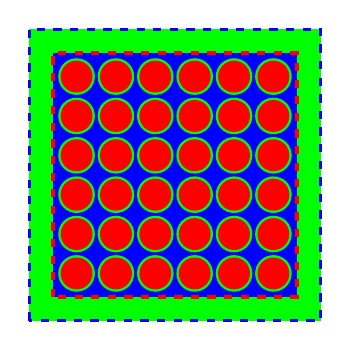
\begin{tikzpicture}[scale=0.5]
            \filldraw[fill=green,draw=blue,very thick,dashed] (-3.7, -3.7) rectangle (3.7, 3.7);
            \filldraw[fill=blue,draw=red,very thick,dashed] (-3.1, -3.1) rectangle (3.1, 3.1);
            \foreach \x in {-2.5,...,2.5}
                \foreach \y in {-2.5,...,2.5} {
                    \filldraw[green,xshift=\x cm,yshift=\y cm] circle (0.45cm);
                    \filldraw[red,xshift=\x cm,yshift=\y cm] circle (0.39cm);
                }
        \end{tikzpicture}
    \end{figure}
\end{frame}

\subsection{Basic settings}

\begin{frame}{Basic settings}
    \begin{itemize}
        \item{Particle counts for criticality calculation}
        \begin{itemize}
            \item{\texttt{set pop <PPC> <ACT> <INACT>}}
        \end{itemize}
        \item{Boundary conditions: 1=vac, 2=ref, 3=periodic}
            \begin{itemize}
                \item{\texttt{set bc <type>}}
                \item{\texttt{set bc <bx> <by> <bz>}}
            \end{itemize}
        \item{Cross sections libraries: \texttt{acelib}}
        \item{Geometry and mesh plotting}
            \begin{itemize}
                \item{\texttt{plot <orientation> <px> <py>}}
                \item{\texttt{mesh <orientation> <px> <py>}}
            \end{itemize}
    \end{itemize}
\end{frame}

\subsection{Processing with \st}

\begin{frame}{Processing with \st}
    \begin{itemize}
        \item{\st contains custom readers and containers}
        \item{Each file type has a dedicated reader for processing, storing data}
        \item{Containers represent objects like detectors, homogenized universes, etc.}
        \item{Easiest way to interact with data: \texttt{serpentTools.read}}
        \item{Store all the data by default}
        \begin{itemize}
            \item{Support for filtering with \texttt{rc} object}
        \end{itemize}
    \end{itemize}
\end{frame}

\section{Expanded Input File}

\begin{frame}{Expanded Input File}
    \tableofcontents[sectionstyle=show/hide,subsectionstyle=show/show/hide]
\end{frame}

\subsection{History settings}

\begin{frame}{History settings}
    \begin{itemize}
        \item Monte Carlo codes compute expected quantities with associated uncertainty
        \item $k_{eff}=1.0009\pm 10 pcm \rightarrow k_{eff} \pm \sigma$
        \item How can we be sure our answer is ``right''?
        \item Some convergence analysis
        \item Increase number of simulated particles $\approx 1/\sqrt{N}$
        \begin{itemize}
            \item 100$\times$ increase for 10\% reduction in uncertainty
        \end{itemize}
    \end{itemize}
\end{frame}

\begin{frame}{History settings}
    \begin{itemize}
        \item Enable detailed cycle-by-cycle output of $k_{eff}$ and entropy
        \item \texttt{set his 1}
        \item \texttt{set entr NX NY NZ}
        \item Examine convergence of criticality and fission source
    \end{itemize}
\end{frame}

\subsection{Detectors}
\begin{frame}{Detectors (tallies)}
    \begin{itemize}
        \item Like MCNP, SERPENT can compute reaction-rate style quantities
        \begin{equation}
            R = \frac{1}{V}\int_\omega\psi(\omega)r(\omega)d\omega
        \end{equation}
        \item $\omega$ can be space and energy domain
        \item Example: one group reaction rates
        \begin{equation}
            r(\omega) = \Sigma_i(E)
        \end{equation}
        \onslide<2->
        \item Many binning options
        \begin{itemize}
            \item energy, reaction, material, xyz mesh, hex mesh, $\cdots$
        \end{itemize}
        \item{Advice: Few detectors with more bins vs. many detectors with few bins}
    \end{itemize}
\end{frame}

\begin{frame}{Detector examples}
    \begin{itemize}
        \item One-group flux tally
        \item Multi-group flux spectrum
        \item Cartesian meshing
        \item Complicated energy, material, reaction, space detector
    \end{itemize}
\end{frame}

\subsection{Depletion}
\begin{frame}{Depletion}
    \begin{itemize}
        \item Process of consuming fuel and producing fission products over time
        \item Typically taken in two steps:
            \begin{enumerate}
                \item Compute flux and power in all burnable materials - $\phi$
                \item Assume $\phi$ is constant and solve Bateman equations $\dot{N}(t)=AN(0)$
            \end{enumerate}
        \item Fixed $\phi$ assumption is valid for \textbf{very small $\Delta t$}
        \item Various coupling schemes improve assumption
            \begin{itemize}
                \item Predictor-corrector, LE/LI, SIE
                \item Substep approach
            \end{itemize}
    \end{itemize}
\end{frame}

\begin{frame}{Depletion settings}
    \begin{itemize}
        \item Must have at least one material specified as burnable
        \begin{itemize}
            \item Set mass or volume of burnable material
        \end{itemize}
        \item SERPENT requires at least two settings:
        \begin{itemize}
            \item Flux normalization
            \item Length of depletion steps
        \end{itemize}
        \item Depletion step can be incremental, or cumulative
        \begin{itemize}
            \item \texttt{dep daystep 1 1 1 1 1}
            \item \texttt{dep daytot 1 2 3 4 5}
        \end{itemize}
        \onslide<2->
        \item Units of burnup, $[MWd/kgU]$
        \begin{itemize}
            \item{\texttt{dep bustep 0.5 1.0 1.0}}
            \item{\texttt{dep butot 0.5 1.5 2.5}}
        \end{itemize}
        \onslide<3->
        \item{Simulate downtime or spent fuel with decay - \texttt{decstep}, \texttt{dectot}}
    \end{itemize}
\end{frame}

\begin{frame}{Depletion ``best'' practices / features}
    \centerline{Personal/community recommendations}
    \begin{itemize}
        \item Always \textbf{always} declare volumes or masses of burnable materials
        \begin{itemize}
            \item Can check with \texttt{-checkvolumes} command
        \end{itemize}
        \item Small steps at beginning to build up initial fission products
        \item Use higher order schemes with substeps \texttt{set pcc LELI 5}
        \item 2 MWd/kgU step length [1 for Gd] with basic schemes
        \begin{itemize}
            \item $\approx$ 5-20 days
        \end{itemize}
        \item Use built in subdivision or manual subdivisions
        \begin{itemize}
            \item \url{http://serpent.vtt.fi/mediawiki/index.php/Automated\_depletion\_zone\_division}
        \end{itemize}
    \end{itemize}
\end{frame}

\section{Specialized SERPENT options}

\begin{frame}{Specialized SERPENT Options}
    \tableofcontents[sectionstyle=show/hide,subsectionstyle=show/show/hide]
\end{frame}

\subsection{Command line tools}

\begin{frame}{SERPENT command line}
    \begin{itemize}
        \item Monte Carlo-based volume checker
        \begin{itemize}
            \item{\texttt{sss2 -checkvolumes <N> <input>}}
        \end{itemize}
        \onslide<2->
        \item Composition indexing
        \begin{itemize}
            \item{\texttt{sss2 -comp list}}
        \end{itemize}
        \onslide<3->
        \item Stochastic particle placement for TRISO/pebble fuel
        \begin{itemize}
            \item{\texttt{sss2 -disperse}}
        \end{itemize}
        \onslide<4->
        \item Track plotter
        \begin{itemize}
            \item{\texttt{sss2 -track <N> <input>}}
        \end{itemize}
    \end{itemize}
\end{frame}

\subsection{Sensitivities}

\begin{frame}{GPT-based Sensitivities}
    \begin{itemize}
        \item Generate sensitivity of parameters to nuclear data
        \begin{itemize}
            \item $S^{k_{eff}}_{\sigma_{capt}^{U8}}\approx
                \frac{\Delta k_{eff}/k_{eff}}{\Delta\sigma^{U8}_{capt} / \Delta\sigma^{U8}_{capt}}$
        \end{itemize}
        \item Void reactivity coefficient
        \item Useful for generating sensitivities to concentrations of specific isotopes
        \onslide<2->
        \item Sensitivity of reaction rate ratios through detectors
        \begin{itemize}
            \item $R\equiv \frac{\int_\omega\phi\sigma_fd\omega}{\int_\omega\phi\sigma_{capt}d\omega}$
            \item $S^R_\sigma\approx\frac{\Delta R/R}{\Delta\sigma /\sigma}$
        \end{itemize}
        \item \url{http://serpent.vtt.fi/mediawiki/index.php/Sensitivity\_calculations}
    \end{itemize}
\end{frame}

\begin{frame}{Sensitivity Settings}
    \begin{itemize}
        \item{What is the response? - \texttt{sens resp}}
        \item{What is perturbed? - \texttt{sens pert}}
        \begin{itemize}
            \item{Nuclear data - \texttt{xs, chi, nubar, eleg}}
            \item{Isotopes - \texttt{zailist}}
            \item{Materials - \texttt{matlist}}
        \end{itemize}
        \item{What energy structure? - \texttt{sens opt egrid}}
    \end{itemize}
\end{frame}

\subsection{Branching calculations}

\begin{frame}{Branching Calculations}
    \begin{itemize}
        \item{Monte Carlo is great, but slow}
        \onslide<2->
        \item{Nodal diffusion is fast, but requires precomputation of homogenized data}
        \begin{itemize}
            \item{Cross sections, kinetic parameters, discontinuity factors, etc}
        \end{itemize}
        \onslide<3->
        \item{Some nodal diffusion codes accept these data across perturbed states}
        \begin{itemize}
            \item{Range of fuel temperatures, coolant densities/temperatures, rod position, etc.}
            \item{Burnup dependence}
        \end{itemize}
    \end{itemize}
\end{frame}

\begin{frame}{Branching Calculations}
    \begin{itemize}
        \item{Use automated branching analysis in SERPENT}
        \item{Can control what goes in the output}
        \item{Wide support for perturbation types}
        \onslide<2->
        \item{Generates a formatted coefficient file}
        \item{\url{http://serpent.vtt.fi/mediawiki/index.php/Automated\_burnup\_sequence}}
    \end{itemize}
\end{frame}

\begin{frame}{\texttt{branches} Dictionary}
    \begin{figure}
        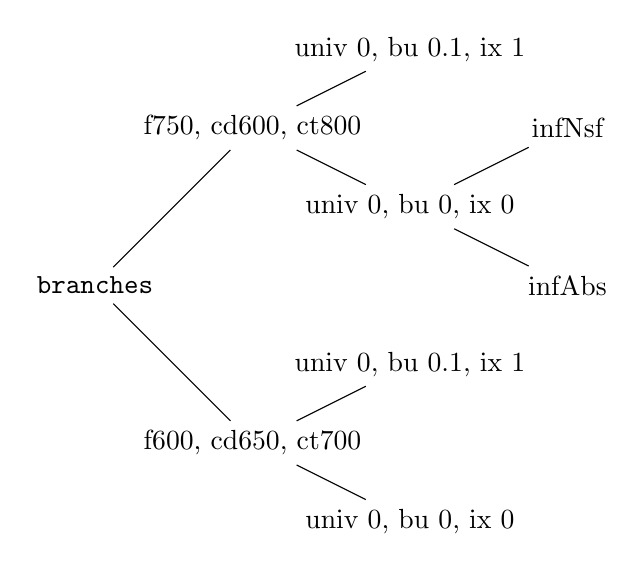
\begin{tikzpicture}[grow=right, level 1/.style={sibling distance=4cm}, level 2/.style={sibling distance=2cm}, level distance=2cm, level 3/.style={sibling distance=2cm}]
            \node {\texttt{branches}}
            child {
                node {f600, cd650, ct700}
                child { node {univ 0, bu 0, ix 0} }
                child { node {univ 0, bu 0.1, ix 1} }
            }
            child {
                node {f750, cd600, ct800}
                child { node {univ 0, bu 0, ix 0}
                    child { node {infAbs} }
                    child { node {infNsf} }
                }
                child { node {univ 0, bu 0.1, ix 1} }
                };
        \end{tikzpicture}
    \end{figure}
\end{frame}

\section{Advanced \st Features}

\begin{frame}{Advanced \st Features}
    \tableofcontents[sectionstyle=show/hide,subsectionstyle=show/show/hide]
\end{frame}

\subsection{Nodal diffusion cross sections}

\begin{frame}{Nodal diffusion cross sections}
    \begin{itemize}
        \item{Tree-like structure may not be ideal}
        \item{Condensed storage, ideal for writing data files for nodal diffusion codes}
        \item{Better storage of cross sections with \texttt{BranchCollector}}
        \begin{itemize}
            \item Pre-release \texttt{0.7.0rc0}
        \end{itemize}
        \item{Support for viewing, and modifying perturbation states}
    \end{itemize}
\end{frame}

\subsection{Control over processed data}

\begin{frame}{Filtering of Processed Data}
    \begin{itemize}
        \item Consider huge output file, result or depletion
        \item Only care about tiny subset of data
        \begin{itemize}
            \item Criticality over time
            \item Atomic density for handful of materials from full core
        \end{itemize}
        \item Use \texttt{serpentTools.settings.rc} settings to control what is processed
        \item{All settings explained \href{https://serpent-tools.readthedocs.io/en/latest/settingsTop.html}{in \texttt{readthedocs} manual}}
    \end{itemize}
\end{frame}

\subsection{Command-line interface}

\begin{frame}{Command-line interface}
    \begin{itemize}
        \item{Modest set of capabilities can be launched from command line}
        \item{\texttt{\$ python -m serpentTools -h}}
        \item{Subcommands for viewing settings, conversion, and seeding files}
    \end{itemize}
\end{frame}

\begin{frame}{Export to MATLAB}
    \begin{itemize}
        \item Many workflows/people prefer MATLAB
        \item Still have to work with large files
        \item Create binary file that can be loaded into MATLAB
        \onslide<2->
        \item Use \st as a compression tool
        \item Take advantage of \st filtering capabilities
        \item \texttt{\$ python -m serpentTools to-matlab dep\_dep.m}
    \end{itemize}
\end{frame}

\begin{frame}{Randomly Seeded Files}
    \begin{itemize}
        \item Common practice with Monte Carlo is to repeat with unique random seeds
        \item Get a handle on the ``true'' uncertainty of system
        \item Reduce effect of stochastic processes
        \onslide<2->
        \item \texttt{\$ python -m serpentTools seed file N}
        \item Generate $N$ new input files with unique random seeds
        \item Support for using \texttt{include} directives to avoid writing whole file
    \end{itemize}
\end{frame}

\section{Integrating with other python modules}

\begin{frame}{Integrating with other python modules}
        \tableofcontents[sectionstyle=show/hide,subsectionstyle=show/show/hide]
\end{frame}

\subsection{\texttt{subprocess}}

\begin{frame}{\texttt{subprocess}}
    \begin{itemize}
        \item{Part of standard library}
        \item{Execute other processes inside of python}
        \item{Capable to build integrated design tool}
        \begin{enumerate}
            \item{Build input files}
            \item{Run SERPENT}
            \item{Scrape output with \st}
        \end{enumerate}
    \end{itemize}
\end{frame}

\subsection{\texttt{scipy}}

\begin{frame}{\texttt{scipy}}
    \begin{itemize}
        \item{Wide-ranging numeric capabilities}
        \item{Sparse matrix support - \texttt{scipy.sparse}}
        \item{Numeric integration - \texttt{scipy.integrate}}
        \item{Optimization routines - \texttt{scipy.optimization}}
    \end{itemize}
\end{frame}

\subsection{\texttt{pandas} and \texttt{seaborn}}
\begin{frame}{\texttt{pandas} and \texttt{seaborn}}
    \begin{columns}
        \column{0.5\textwidth}
        \begin{itemize}
            \item{Data analysis tool kit}
            \item{Excellent tabulated data framework}
            \item{I/O to csv, hdf5, Excel, etc}
        \end{itemize}

        \column{0.5\textwidth}
        \begin{itemize}
            \item{Powerful plotting library}
            \item{Deep-dive into underlying data}
        \end{itemize}
    \end{columns}
\end{frame}


\section*{Outro}

\begin{frame}{Conclusion}
    \begin{itemize}
        \item Walked through a wide variety of SERPENT settings and examples
        \item Processed the data using \st
        \item More complicated analysis built using \st API
    \end{itemize}
\end{frame}

\begin{frame}{What next?}
    \begin{itemize}
        \item{Dive right in!}
        \item{Interested in updates?}
        \begin{itemize}
            \item{Mailing list - \url{https://pwp.gatech.edu/core/contact-us/}}
            \item{Follow the repository on Github}
        \end{itemize}
        \item{Interested in developing?}
        \begin{itemize}
            \item{Happily welcome contributors}
            \item{Developer's guide - \url{https://serpent-tools.readthedocs.io/en/latest/develop/index.html}}
            \item{Search for ``good first issue'' or ``help wanted'' on \href{https://github.com/CORE-GATECH-GROUP/serpent-tools/issues}{Issue Tracker}}
        \end{itemize}
    \end{itemize}
\end{frame}

\begin{frame}{Conclusion}
    \begin{itemize}
        \item{Thank you very much!}
        \item{My github: \href{https://github.com/drewejohnson}{\texttt{drewejohnson}}}
        \item{Any questions?}
    \end{itemize}
\end{frame}

\end{document}
